% ----------------------------------------------------------------
% Report Class (This is a LaTeX2e document)  *********************
% ----------------------------------------------------------------
\documentclass[11pt]{report}
\usepackage[english]{babel}
\usepackage{amsmath,amsthm}
\usepackage{amsfonts}
\usepackage{amssymb}%
\usepackage{graphicx}%
\usepackage{tabularx}
\usepackage{epstopdf}

\addtolength{\textheight}{3.2cm}
\addtolength{\textwidth}{2cm}
\addtolength{\marginparwidth}{-2.2cm}
\addtolength{\oddsidemargin}{-1.4cm}
\addtolength{\headheight}{-2.4cm}
%\addtolength{\footskip}{-6cm}

% THEOREMS -------------------------------------------------------
\newtheorem{thm}{Theorem}[chapter]
\newtheorem{cor}[thm]{Corollary}
\newtheorem{lem}[thm]{Lemma}
\newtheorem{prop}[thm]{Proposition}
\theoremstyle{definition}
\newtheorem{defn}[thm]{Definition}
\theoremstyle{remark}
\newtheorem{rem}[thm]{Remark}
% ----------------------------------------------------------------
\begin{document}

%\title{STATS 782, 2017}
\setlength\extrarowheight{3pt}
\begin{tabular*}{\textwidth}{ @{} l @{\extracolsep\fill} c @{\extracolsep\fill} r @{}}
  \hline
  % after \\: \hline or \cline{col1-col2} \cline{col3-col4} ...
  \textbf{STATS 782, 2017} & \textbf{Assignment1} & \textbf{Date: 2017-08-15} \\
   & Zhi Zhang, 708439475, zzha822 & \\
  \hline
\end{tabular*}
%\author{Zhi Zhang, $\ $708439475, $\ $zzha822
%\\The University of Auckland}
%\date{August 3, 2017}
%\maketitle

\begin{enumerate}
    \item[1.] The answers are below:
    \begin{verbatim}> fib = function(n) {
+   s = numeric(n)
+
+   if (n <= 1) s[n] = 0
+   else {
+     s[1:(n - 1)] = fib(n - 1)
+     if (n == 2) s[n] = 1
+     else s[n] = s[n - 1] + s[n - 2]
+   }
+
+   s
+ }
>
> fib(1)
[1] 0
> fib(2)
[1] 0 1
> fib(3)
[1] 0 1 1
> fib(10)
 [1]  0  1  1  2  3  5  8 13 21 34\end{verbatim}

    \item[2.] The answers are below:
    \begin{enumerate}
    	\item[(a)] \begin{verbatim}> clusters.medians = function(x, c) {
+   lenc = length(c)
+
+   d = outer(c, x, function(cj, xi) abs(xi - cj))
+   d.minnum = apply(d, 2, which.min)
+
+   con = outer(1:lenc, d.minnum, function(num, minnum) num == minnum)
+
+   xv = unlist(apply(con, 1, function(t) median(x[t])))
+   xv
+ }
>
> find.clusters.medians = function(x, c) {
+   ctmp1 = c
+   repeat {
+     ctmp2 = clusters.medians(x, ctmp1)
+     if (all(abs(ctmp1 - ctmp2) < 1e-07)) break
+     else ctmp1 = ctmp2
+   }
+   ctmp1
+ }
>
> x = faithful$eruptions
> find.clusters.medians(x, c(2,4))
[1] 1.9830 4.3415\end{verbatim}
 	\item[(b)] \begin{verbatim}> find.clusters.medians(x, c(2,3,4))
[1] 1.9830 3.9665 4.5330\end{verbatim}
 	\item[(c)] \begin{verbatim}> find.clusters.medians(x, c(2,3,4,5))
[1] 1.967 3.600 4.150 4.600\end{verbatim}
    \end{enumerate}

    \item[3.] The answers are below:
    \begin{verbatim}> sign.matrix = function(x) outer(x, x, function(x1, x2) sign(x1 - x2))
>
> conc = function(x, y) {
+   conc.mtx = sign.matrix(x)
+   conc.mty = sign.matrix(y)
+   conc.z = conc.mtx + conc.mty
+   c = length(which(conc.z < 0 | conc.z > 0))
+   n = length(x)
+   c / (n * (n - 1))
+ }
>
> conc(x = 1:5, y = c(3, 1, 4, 5, 2))
[1] 0.6
>
> set.seed(782)
> x = round(rnorm(1000))
> y = x + round(rnorm(1000))
> conc(x, y)
[1] 0.8518939\end{verbatim}
 	
    \item[4.] The answers are below:
    \begin{enumerate}
    	\item[(a)] \begin{verbatim}> nba.df = read.csv("https://raw.githubusercontent.com/
zzdxzhangzhi/assignments/master/782/NBA2016-2017.csv",
+ stringsAsFactors = FALSE)
> names(nba.df) = c("team1", "team2", "wins")
> head(nba.df)
          team1               team2 wins
1 Atlanta Hawks      Boston Celtics    2
2 Atlanta Hawks       Brooklyn Nets    2
3 Atlanta Hawks   Charlotte Hornets    1
4 Atlanta Hawks       Chicago Bulls    3
5 Atlanta Hawks Cleveland Cavaliers    3
6 Atlanta Hawks    Dallas Mavericks    2
> 
> nba.names = nba.df$team1[seq(1, 870, length = 30)]
> nba.names
 [1] "Atlanta Hawks"          "Boston Celtics"         "Brooklyn Nets"
          "Charlotte Hornets"     
 [5] "Chicago Bulls"          "Cleveland Cavaliers"    "Dallas Mavericks"
       "Denver Nuggets"        
 [9] "Detroit Pistons"        "Golden State Warriors"  "Houston Rockets"
        "Indiana Pacers"        
[13] "Los Angeles Clippers"   "Los Angeles Lakers"     "Memphis Grizzlies"
      "Miami Heat"            
[17] "Milwaukee Bucks"        "Minnesota Timberwolves" "New Orleans Pelicans"
   "New York Knicks"       
[21] "Oklahoma City Thunder"  "Orlando Magic"          "Philadelphia 76ers"
     "Phoenix Suns"          
[25] "Portland Trail Blazers" "Sacramento Kings"       "San Antonio Spurs"
      "Toronto Raptors"       
[29] "Utah Jazz"              "Washington Wizards"    
> log.likelihood.r = function(r, times, s) {
+   rn = s - sum(r)
+   rr = c(r, rn)
+   
+   if (all(rr > 0)) {
+     mtx = outer(rr, rr, function(ri, rj) log(ri / (ri + rj)))
+     rankv = c(t(mtx)[which(row(mtx) != col(mtx))])
+     sum(times * rankv)
+   } else {
+     -Inf
+   }
+ }
> 
> s = 1000
> Q = function(r) {
+   -log.likelihood.r(r, nba.df$wins, s)
+ }
> 
> count = length(nba.names)
> result = optim(seq(1, 29, length = 29), Q, method = "BFGS", 
+                control = list(maxit = 200))
> result
$par
 [1]  28.920344  49.262769   8.487427  20.865839  26.562360  
45.009903  18.735556  26.484090  21.994617
[10] 127.851303  59.221865  27.412854  47.775175  12.710449  
32.153364  26.968452  28.090105  17.226476
[19]  19.848702  15.942769  38.873109  14.320608  13.473253  
11.341333  28.116503  17.982849  83.968346
[28]  43.789158  47.019261

$value
[1] 761.4917

$counts
function gradient 
     147      143 

$convergence
[1] 0

$message
NULL

> 
> ratio = 100 / result$par[which.max(result$par)]
> r.value = result$par * ratio
> rr.value = c (r.value, (s - sum(result$par)) * ratio)
> rr.value
 [1]  22.620297  38.531300   6.638514  16.320396  20.775979  
35.204884  14.654177  20.714760  17.203279
[10] 100.000000  46.320893  21.441200  37.367766   9.941587  
25.149031  21.093608  21.970918  13.473837
[19]  15.524833  12.469774  30.404938  11.200987  10.538221   
8.870722  21.991566  14.065441  65.676566
[28]  34.250068  36.776521  30.966569
> 
> rank.table = data.frame(nba.names, rr.value, stringsAsFactors = FALSE)
> ordered.rank = rank.table[order(rank.table$rr.value, decreasing = TRUE),]
> colnames(ordered.rank) = c("name", "rank")
> rownames(ordered.rank) = 1:30
> ordered.rank
                     name       rank
1   Golden State Warriors 100.000000
2       San Antonio Spurs  65.676566
3         Houston Rockets  46.320893
4          Boston Celtics  38.531300
5    Los Angeles Clippers  37.367766
6               Utah Jazz  36.776521
7     Cleveland Cavaliers  35.204884
8         Toronto Raptors  34.250068
9      Washington Wizards  30.966569
10  Oklahoma City Thunder  30.404938
11      Memphis Grizzlies  25.149031
12          Atlanta Hawks  22.620297
13 Portland Trail Blazers  21.991566
14        Milwaukee Bucks  21.970918
15         Indiana Pacers  21.441200
16             Miami Heat  21.093608
17          Chicago Bulls  20.775979
18         Denver Nuggets  20.714760
19        Detroit Pistons  17.203279
20      Charlotte Hornets  16.320396
21   New Orleans Pelicans  15.524833
22       Dallas Mavericks  14.654177
23       Sacramento Kings  14.065441
24 Minnesota Timberwolves  13.473837
25        New York Knicks  12.469774
26          Orlando Magic  11.200987
27     Philadelphia 76ers  10.538221
28     Los Angeles Lakers   9.941587
29           Phoenix Suns   8.870722
30          Brooklyn Nets   6.638514
>  \end{verbatim}
 	    \item[(b)] \begin{verbatim}> log.likelihood.r.deriv = function(r, i, times1, times2) {
+   rlen = length(r)
+   
+   if (all(r > 0)) {
+     mtx1 = outer(r[i], r[-i], function(ri, rj) rj / ri * (ri + rj))
+     mtx2 = outer(r[i], r[-i], function(ri, rj) 1 / (ri + rj))
+     deriv1 = c(t(mtx1), 
+                1 / r[i]) * times1[(rlen * (i - 1) + 1) : (rlen * i)]
+     deriv2 = c(t(mtx2), 
+                1 / (s - sum(r))) * times2[(rlen * (i - 1) + 1) : (rlen * i)]
+     
+     sum(deriv1) - sum(deriv2)
+   } else {
+     -Inf
+   }
+ }
> 
> Q.derivs = function(r) {
+   order.team2 = order(nba.df$team2)
+   wins.team2 = nba.df$wins[order.team2]
+   rlen = length(r)
+   gradients = numeric(rlen)
+   for (i in 1:rlen) {
+     gradients[i] = log.likelihood.r.deriv(r, i, nba.df$wins, wins.team2)
+   }
+   
+   gradients
+ }
> 
> result.deriv = optim(seq(1, 29, length = 29), Q, gr = Q.derivs, 
+                      method = "BFGS")
> result.deriv
$par
 [1]  1  2  3  4  5  6  7  8  9 10 11 12 13 14 15 16 17 18 19 
20 21 22 23 24 25 26 27 28 29

$value
[1] 1109.275

$counts
function gradient 
      29        1 

$convergence
[1] 0

$message
NULL

> \end{verbatim}
 	    \item[(c)] \begin{verbatim}> ranks = c(result$par, s - sum(result$par))
> ranks.sort = sort(ranks, decreasing = TRUE)
> first2 = c(which(round(ranks) == round(ranks.sort[1])), 
+            which(round(ranks) == round(ranks.sort[2])))
> first2
[1] 10 27
> 
> Q2 = function(r1, r2) {
+   m = max(length(r1), length(r2))
+   if (length(r1) < m)
+     r1 = rep(r1, length = m)
+   if (length(r2) < m)
+     r2 = rep(r1, length = m)
+   
+   ans = numeric(m)
+   for (i in 1:m) {
+     ranks[first2] = c(r1[i], r2[i])
+     ans[i] = -log.likelihood.r(ranks[-length(ranks)], nba.df$wins, s)
+   }
+   
+   ans
+ }
> 
> r1 = seq(40, 145, length = 61)
> r2 = seq(20, 100, length = 61)
> z = outer(r1, r2, Q2)
> contour(r1, r2, z,
+         xlab = paste("rank of", nba.names[first2[1]]),
+         ylab = paste("rank of", nba.names[first2[2]]))
> \end{verbatim}
    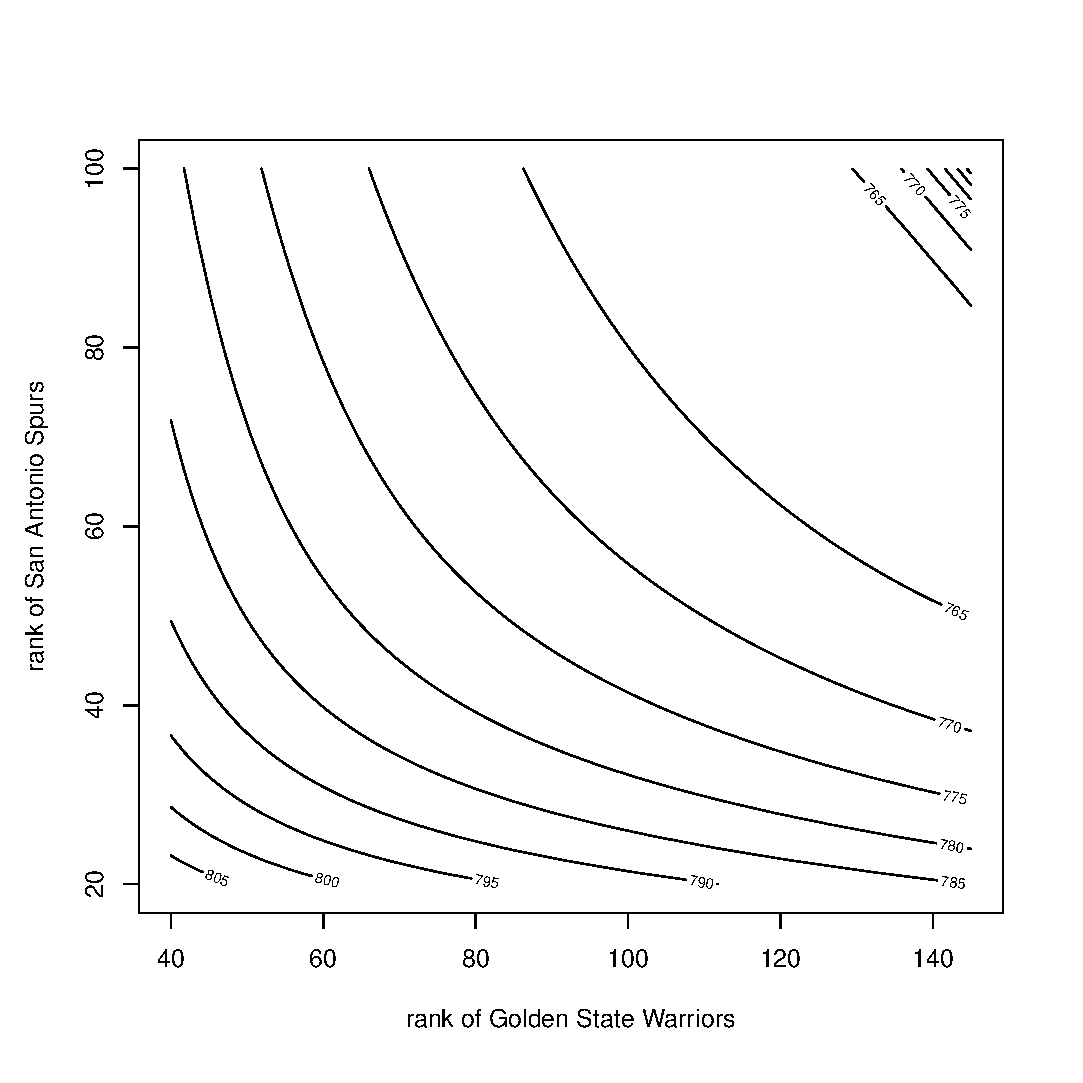
\includegraphics[width=\textwidth]{a2_contour.eps}
    \begin{verbatim}> r1 = seq(40, 145, length = 1001)
> r2 = seq(20, 100, length = 6)
> z = outer(r1, r2, Q2)
> par(mfrow = c(2, 3))
> ran = range(z)
> for(j in 1:length(r2)) {
+   plot(r1, z[, j], ylim = ran, type = "l",
+        main = paste("rank of", 
+                     nba.names[first2[2]], 
+                     "=", 
+                     r2[j]),
+        xlab = paste("rank of", nba.names[first2[1]]),
+        ylab = "Q")
+ }
> \end{verbatim}
   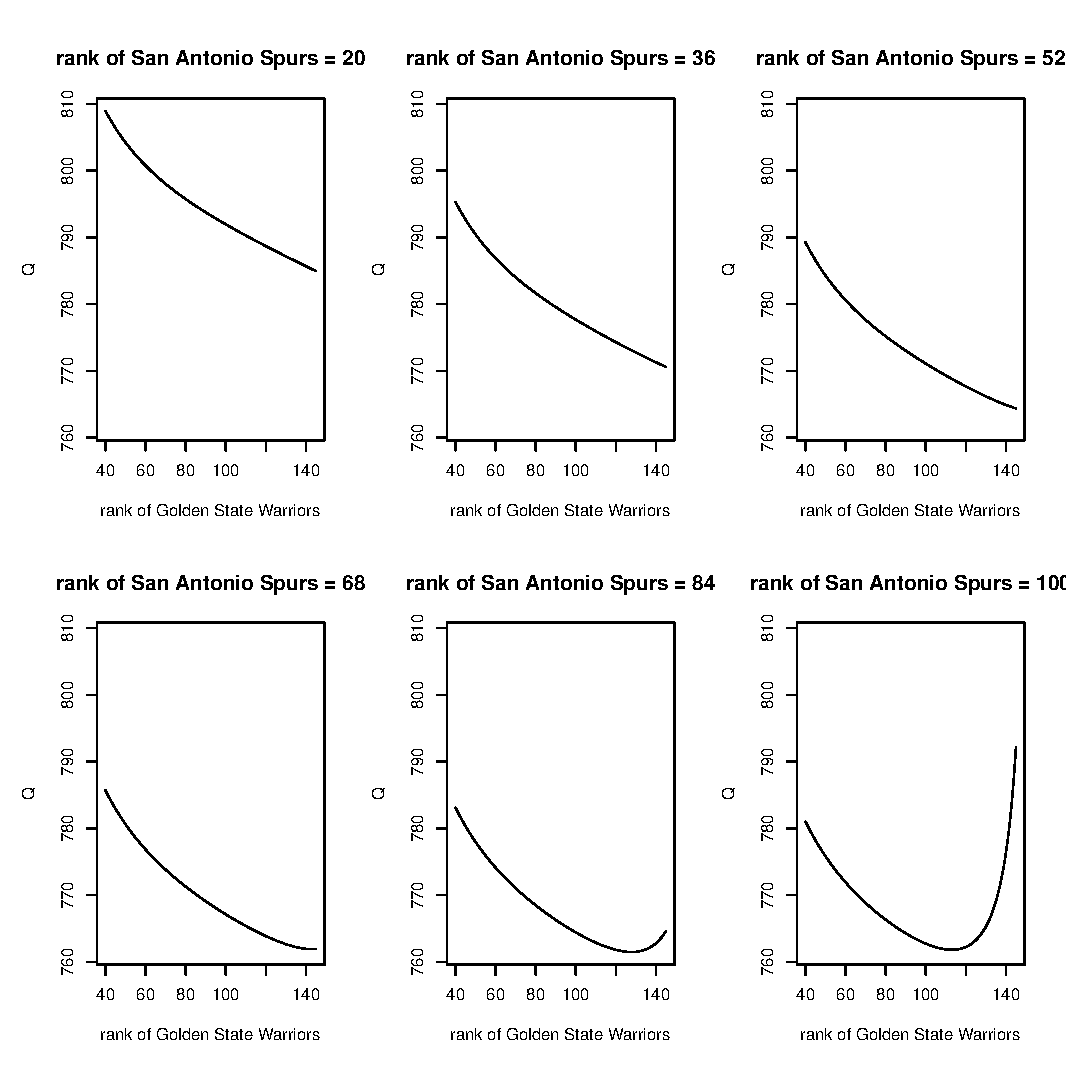
\includegraphics[width=\textwidth]{a2_profile.eps}
    \end{enumerate}

\end{enumerate}

\end{document}
% ----------------------------------------------------------------
